%
% The first command in your LaTeX source must be the \documentclass command.
\documentclass[sigconf]{acmart}

\usepackage{multirow}
\usepackage[linesnumbered,ruled]{algorithm2e}
\usepackage{algpseudocode}
\usepackage{citeall}
\renewcommand{\algorithmicrequire}{\textbf{Input:}} % Use Input in the format of Algorithm
\renewcommand{\algorithmicensure}{\textbf{Output:}} % Use Output in the format of Algorithm
%
% defining the \BibTeX command - from Oren Patashnik's original BibTeX documentation.
\def\BibTeX{{\rm B\kern-.05em{\sc i\kern-.025em b}\kern-.08emT\kern-.1667em\lower.7ex\hbox{E}\kern-.125emX}}
    
% Rights management information. 
% This information is sent to you when you complete the rights form.
% These commands have SAMPLE values in them; it is your responsibility as an author to replace
% the commands and values with those provided to you when you complete the rights form.
%
% These commands are for a PROCEEDINGS abstract or paper.
\copyrightyear{2019}
\acmYear{2019}
\setcopyright{acmlicensed}
\acmConference[KDD '19]{KDD '19: The 24th ACM SIGKDD International Conference on Knowledge
	Discovery \& Data Mining}{August 04--08, 2019}{Anchorage, Alaska - USA}
\acmBooktitle{KDD '19: The 24th ACM SIGKDD International Conference on Knowledge
	Discovery \& Data Mining, August 04--08, 2019, Anchorage, Alaska - USA}
\acmPrice{15.00}
\acmDOI{10.1145/1122445.1122456}
\acmISBN{978-1-4503-9999-9/18/06}

%
% These commands are for a JOURNAL article.
%\setcopyright{acmcopyright}
%\acmJournal{TOG}
%\acmYear{2018}\acmVolume{37}\acmNumber{4}\acmArticle{111}\acmMonth{8}
%\acmDOI{10.1145/1122445.1122456}

%
% Submission ID. 
% Use this when submitting an article to a sponsored event. You'll receive a unique submission ID from the organizers
% of the event, and this ID should be used as the parameter to this command.
%\acmSubmissionID{123-A56-BU3}

%
% The majority of ACM publications use numbered citations and references. If you are preparing content for an event
% sponsored by ACM SIGGRAPH, you must use the "author year" style of citations and references. Uncommenting
% the next command will enable that style.
%\citestyle{acmauthoryear}

%
% end of the preamble, start of the body of the document source.
\begin{document}

%
% The "title" command has an optional parameter, allowing the author to define a "short title" to be used in page headers.
\title{A FAX Ingestion Solution with Deep Learning for Financial Institutions}

\begin{comment}
	Financial institution fax solution means: 
	1. large scale
	2. wide variety in layout pattern

\end{comment}

%
% The "author" command and its associated commands are used to define the authors and their affiliations.
% Of note is the shared affiliation of the first two authors, and the "authornote" and "authornotemark" commands
% used to denote shared contribution to the research.
\author{Han Fu}
\email{11821003@zju.edu.cn}
\affiliation{%
  \institution{Zhejiang Unnversity}
  \city{Hangzhou}
  \country{China}
}

\author{Zhuo Li}
\email{Zhuo_Li@statestreet.com}
\affiliation{%
  \institution{State Street}
  \city{Hangzhou}
  \country{China}}
%
% By default, the full list of authors will be used in the page headers. Often, this list is too long, and will overlap
% other information printed in the page headers. This command allows the author to define a more concise list
% of authors' names for this purpose.

%
% The abstract is a short summary of the work to be presented in the article.
\begin{abstract}
In this paper, we introduce the large scale fax recognition system in State Street. To be specific, we divide the complicated coupled task into three subtasks. First, we detect the handwritten signatures and verify whether the handwrittings are authorized or not. The detection model is based on Faster-RCNN and the handwriting verification model consists of a deep convolutional neural network and an angular-softmax output layer. Second, we build a convolutional image classification model to identify which company or functional category the fax belongs to. Finally, detailed contents of interest are extracted by a text recognition system, which contains two components, a light-head R-CNN model is responsible for detecting the locations of each cell in tables and each text snippet, and a Convolutional Recurrent Nueral Network (CRNN) is leveraged for OCR. We conduct abundant experiments on both synthetic and real-world data in State Street. The experimental results indicate the effectiveness and efficiency of our methods.

\end{abstract}

%
% The code below is generated by the tool at http://dl.acm.org/ccs.cfm.
% Please copy and paste the code instead of the example below.
%

%
% Keywords. The author(s) should pick words that accurately describe the work being
% presented. Separate the keywords with commas.
\keywords{data recognition, data detection, signature verification, neural networks}

%


%
% This command processes the author and affiliation and title information and builds
% the first part of the formatted document.
\maketitle

\section{Introduction}
Fax has played an important role in business world to share files remotely since the introduction of the first commercialized version of modern fax machines in 1964 by Xerox Corporation. After we entered 21st century, people may have an intuitive impression that FAX usage is reduced due to increasing competition from Internet-based alternatives like emails, but the reality is it is as important to business as it ever was, if not more. According to \cite{couponchili2015faxfacts}, there are 46.3 million Fax machines in the world, who sent 16 billion faxes in 2017. That means a big financial and environmental cost. Nevertheless, according to \cite{idc2017faxusagewhitepaper}, 82\% of survey respondents said fax usage increased of the past year, and they expect it to continue growing by another 25\% over the next two years. Multiple reasons involved make reducing Fax usage a challenge.
1. regulation and government standards allow and encourage faxing. Technically an e-signature might be enough for somebody, but the legality of an e-signature can't be intuitively recognized and accepted. Many people just don't want to take the risk;
2. many believe fax is more secure than email. Technically a secure email can also save you from malware and ransomware but it is much expensive than a fax machine;
3. fax can provide a complete trail including confirmations of document receipt. This provides extra strengthen for communication resiliency;

Due to these factors, fax still has a massive user base and becomes too prevalent to walk away. Financial industry probably is one of the few most heavy fax users as its strictly regulated nature. In financial industry, fax ingestion usually involves 3 steps: fax classification, signature verification and data extraction. The whole process is very manual and error-prone. Most of time it involves hard copies printed out, which engages extra overhead in document retention, disposal and archiving as well. Data representation and layout variability across faxes make it extremely challenging to find a solution to validate data integrity and transform data into easy to manage knowledge.  Besides all these challenges, there are other challenges preventing improvement of fax file processing automation level:
1. fax image quality could vary widely for different reasons. Sometimes it is a "refaxed" version which reduced the quality, sometimes the fax machine itself may run out of ink;
2. unstructured fax content requires more efforts to extract useful information distributed in it;
3. handwritings on fax files require technologies like OCR and NLP to either verify its integrity or understand its semantics. Examples include handwritten signatures and comments on faxes;


In this paper, we focus on an end to end solution for financial fax file ingestion to improve overall operation efficiency with less human intervention with above challenges in mind. At its core, it has trainable machine learning models fitting different steps in fax ingestion. These models are integrated with fax processing system via a set of RESTFUL APIs. A microservice framework is designed for scalability consideration. Both online and offline trainings are supported via a managed sample set and correctional user feedbacks.
 
The rest of this paper is structured as follows: Section 2 introduces state-of-art fax ingestion solutions. In section 3, we present the overall design of the solution and its components. Section 4 discusses in specific how deep learning is employed towards an accurate and efficient signature verification, with experiment proofs. Section 5 discusses in details how content ingestion and data extractions are done with experiment proofs. In section 6, we deploy our solution for a real life financial institution to resolve its fax processing challenges. Specific performance tuning is done for it and incremental learning is designed for a continuously evolving model. Last but not the least, in section 7, we discuss open questions w.r.t research and possible next steps for this solution.

\begin{comment}
new structure of the paper will like below
2. 介绍传真识别问题域的研究现状
3. 系统整体设计
4. 签名校验模块中的深度学习
5. 内容萃取(ingestion)和结构数据抽取中的深度学习
6. 生产环境部署
        介绍案例的背景
        a. 在线与离线学习
        b. 性能调优
        c. 部署策略
7. Conclusion and Future Works
Acknowledgements
\end{comment}

\section{Related Works}
The problem of data extraction from documents images has drawn attention over decades \cite{nagy2000twenty}, and is where most traditional fax ingestion solutions fall into. Generally, it involves two types of tasks: text recognition and document parsing. With the application of deep neural networks, OCR engines such as Tesseract \cite{smith2007overview} have achieved good performance in dealing documents with simple textual layouts. \cite{jaderberg2014synthetic} firstly employ convolutional neural networks to extract text features and train end-to-end learnable recognition models. Following this work, several advanced approaches were proposed. Broadly speaking, these approaches can be categorized into two types: separated text detection and recognition processes like \cite{shi2017end, tian2016detecting, he2017deep, lyu2018multi, borisyuk2018rosetta}, or joint text detection and recognition processes such as \cite{li2017towards, buvsta2017deep, liu2018fots}. Besides, there are some works concentrating on extracting document data directly into structured formats \cite{cesarini1998informys, chanod2005legacy, peanho2012semantic, li2016precomputed}. However, such works usually needs accurate textual information and expertise knowledge from users, which constrains their adaptibility in extraing data from images.

\begin{comment}
传统的图像内容抽取解决方案关注的重点是把图片或者可编程的文档转化成文本,对于识别真正有意义的数据元素并将他们映射到合理的数据结构中并不是终点。但对于金融机构日常处理的大部分传真文件来说,他们关注的重点只是其中一部分的信息 - 比如说成交价格、日期,机构的运营人员 需要把这些信息萃取出来之后,注射到现有的处理系统让他们数字化地流动。
\end{comment}

On the other hand, for most fax documents financial institutions process everyday, only limited data elements are concerned rather than the whole document, for example, order prices, trade date, etc. Operators from institutions will ''ingest'' and ''inject'' them into application systems. But most existing fax recognition works focus on converting programmatic documents (i.e., PDF) or images into text as a whole with all format details captured (font size, charater directions, etc.), leaving the task of precise data ingestion a lower priority. That's why there is no ''complete'' fax processing solution in financial industry yet - they only resolve the ''conversion'' problem, but not the ''ingestion'' problem which is the ultimate demand. With all above challenges in mind, we try to find a solution for financial fax processing by weighting data ingestion more over format. We spot signatures and tabular data with more focus, as the former is at the critical path beginning of fax processing, and the later stand for most efficiency improvement opportunity to capture concerned data elements in a batch. The solution requires a robust and accurate object detection model, where a few methods have been developed \cite{ren2015faster, dai2016r, li2017light}. We choose Faster R-CNN \cite{ren2015faster} to detect signatures and Light-Head R-CNN \cite{li2017light} to capture tabular data respectively. 

Besides the high performance, the reason we choose deep neural network-based methods in our system is models can be finetuned to fit the new coming data via backpropagation, which is natural for a online system. There exists several researches working on incrementally improving trained models with online data such as \cite{shmelkov2017incremental, su2016line}. Inspired by such works, we design an interactive learning strategy to train online models with author feedbacks and avoid the catastrophic forgetting problem.

\section{Solution Overview}
\subsection{Solution Architecture}

\begin{figure}[h]
	\centering
	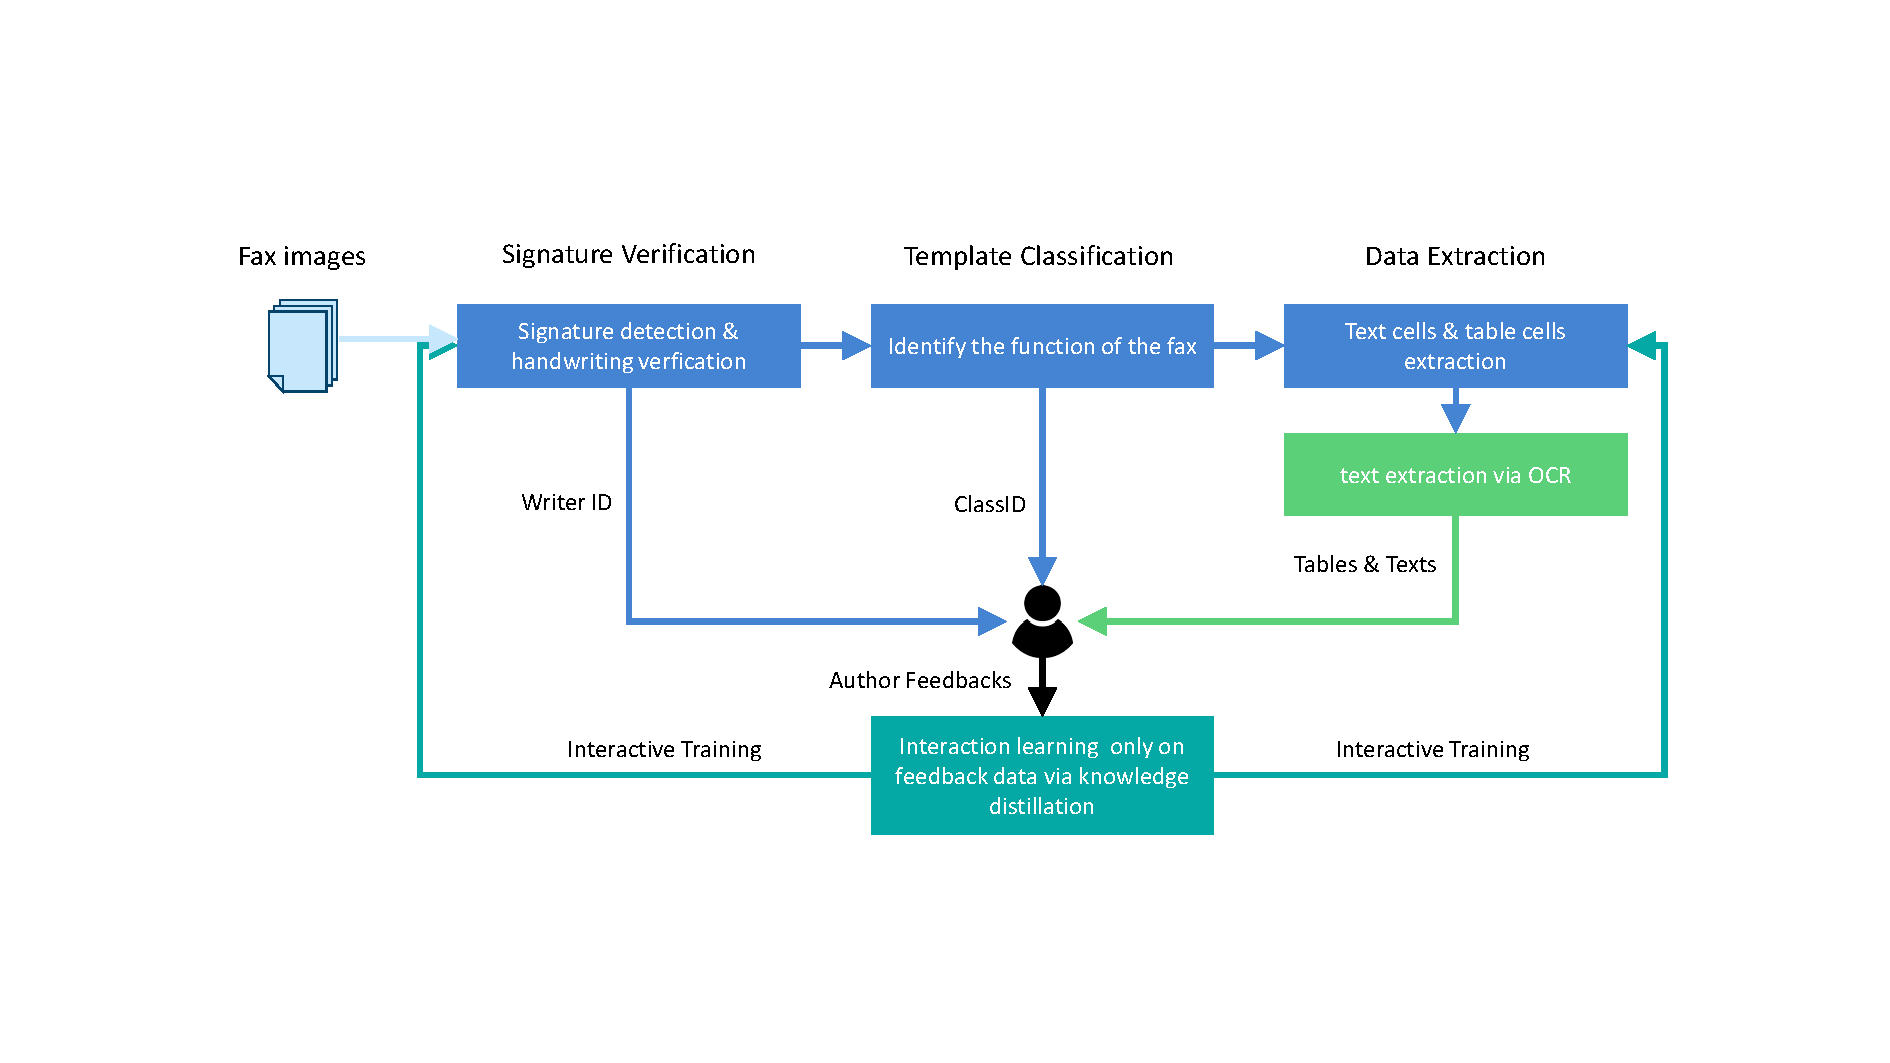
\includegraphics[width=\linewidth]{figure1}
	\caption{Solution Architecture Overview. }
	\label{figure1}
\end{figure}

The solution architecture overview is shown in Figure \ref{figure1}. It consists of three major components, with respect to fax processing workflow in real financial institutions - signature verification, template classification and data extraction.

Most financial FAX documents have hand-written signatures inside from senders (just cover page or every page) as a proof of truth. At the very beginning of processing, these signatures need to be verified before further processing. Signature verification component firstly locates possible signatures on FAX documents via an object detection model, then feeds detected area(s) to a handwritting verification model. We treat this problem as a classification problem rather than a handwriting conversion problem as signatures could be forged but handwriting features won't change easily. Each authorized sender will be pre-collected with a class ID assigned. Detected signature areas will be classified into class IDs ranked by possibility. 

The second component classifies FAXes into different templates which are pre-trained based on layout and sender information. A template contains multiple function areas which can be mapped to structured data formats jointly. Note that we do not set the detail location of each area but only give a semantic label as classification result, which indicates more on the targeted structured data formats rather than Fax document landscape, as FAX documents are not always upright due to twists introduced when faxing source files. The concrete area spotting and data extraction are accomplished in the third component.

The last component is the data extraction piece. It serves two main goals. First, another object detaction model is trained to locate rectangle areas of concerned text paragraphs or tabular data. The second step is to further recognize detail data elements from either text paragraph or tabular datarows. 

The whole process is conducted semi-automatically as it is too risky to allow full straight through processing in FAX ingestion when FAX document quality is impacted by many factors. A UI is provided for operational staff to review and edit results. At every step where manual check is involved, any correction made will be included into the ground truth training sample set, fed into relative incremental training process to continuously refine the model.

\subsection{Training strategy}
For model training's efficiency and effectiveness concern, we propose a staged training strategy inspired by \cite{bengio2009curriculum}. A large amount of mock data are synthesized with similar data structure in real faxes but a much simpler layout. Once models are converged, we set initialization weights on them and further train them with more complex real scenario like layouts - we call them ''true'' faxes. This easy-to-hard training strategy makes model converging process faster. \ref{figure4} shows both initial synthesized fax and further complicated fasx for data extraction task.

\begin{figure}[h]
	\centering
	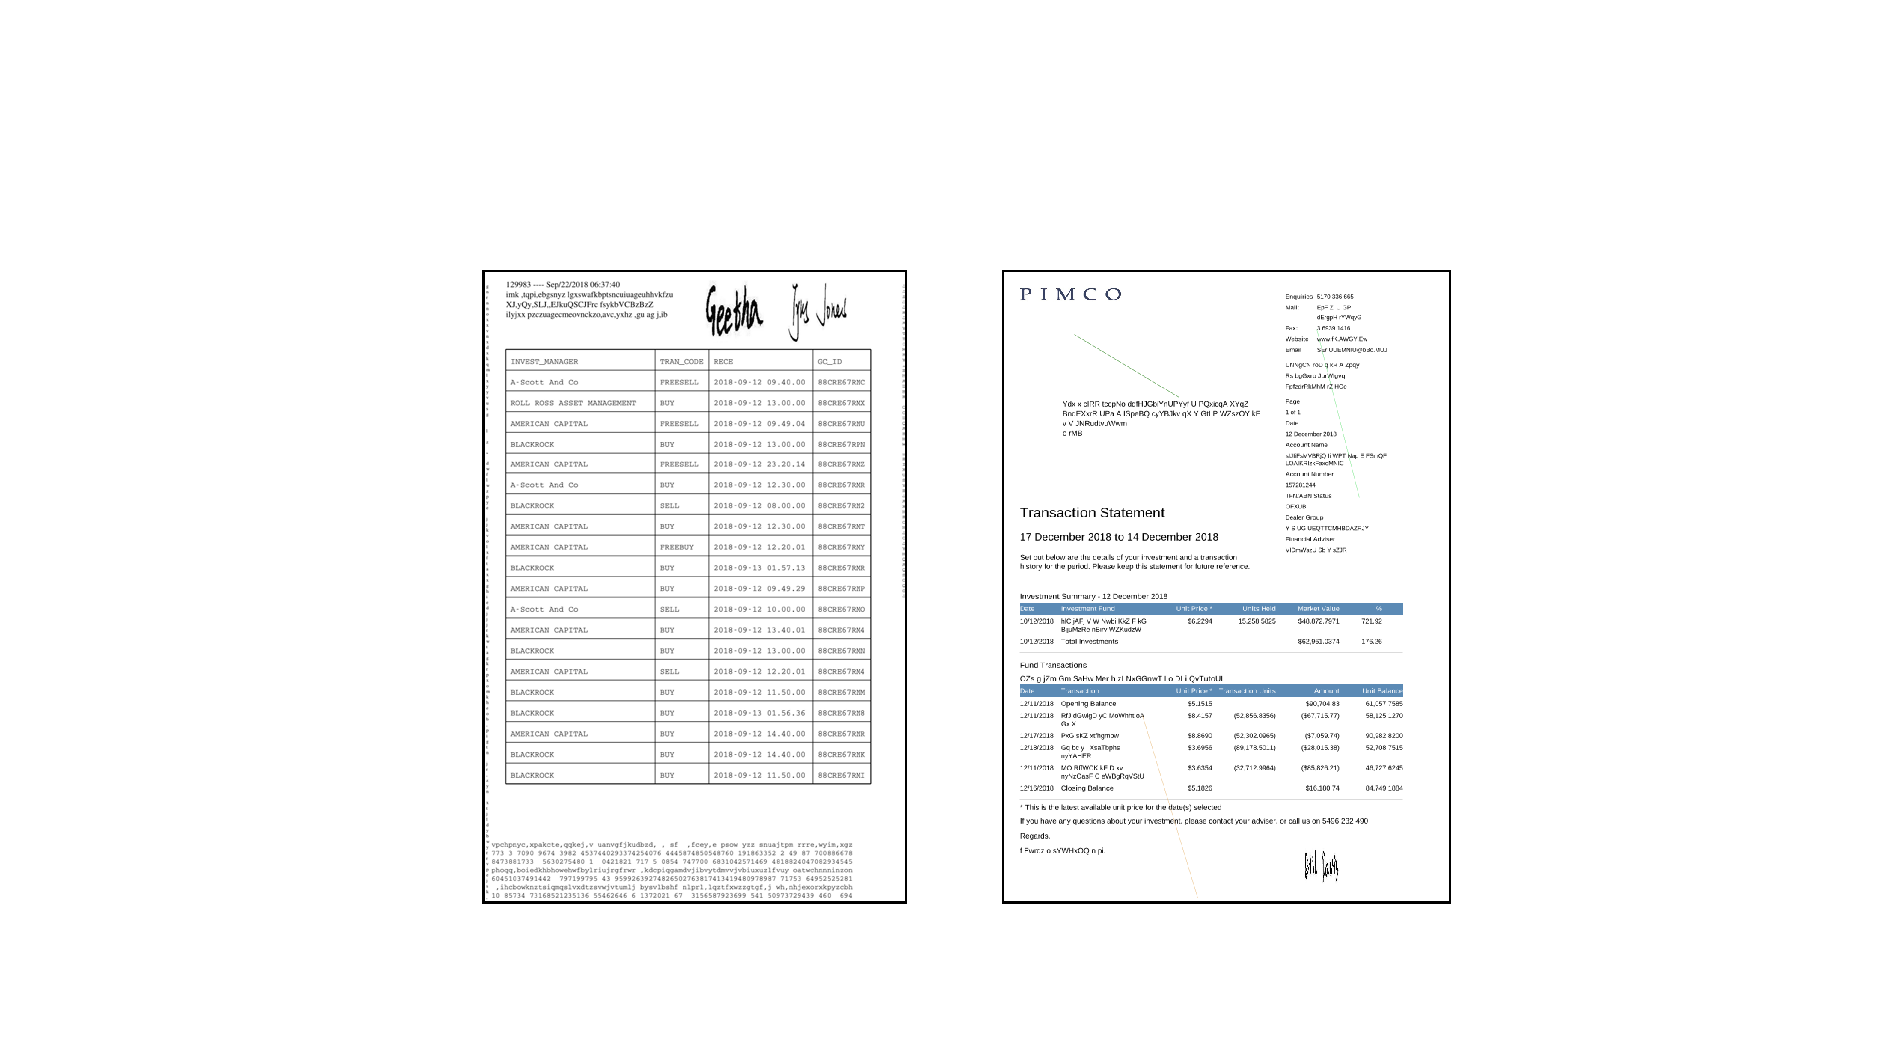
\includegraphics[width=\linewidth]{figure4}
	\caption{Comparison between synthesized fax (left) and a real one (right) on the data extraction task. }
	\label{figure4}
\end{figure}

\section{Signature Verification}

As introduced above, signature verification is at the very beginning of the whole FAX processing crtical path. It can be divided into two steps: first, detect signatures and crop them from FAX document; second, map signatures into authorized names.

\begin{figure*}[h]
	\centering
	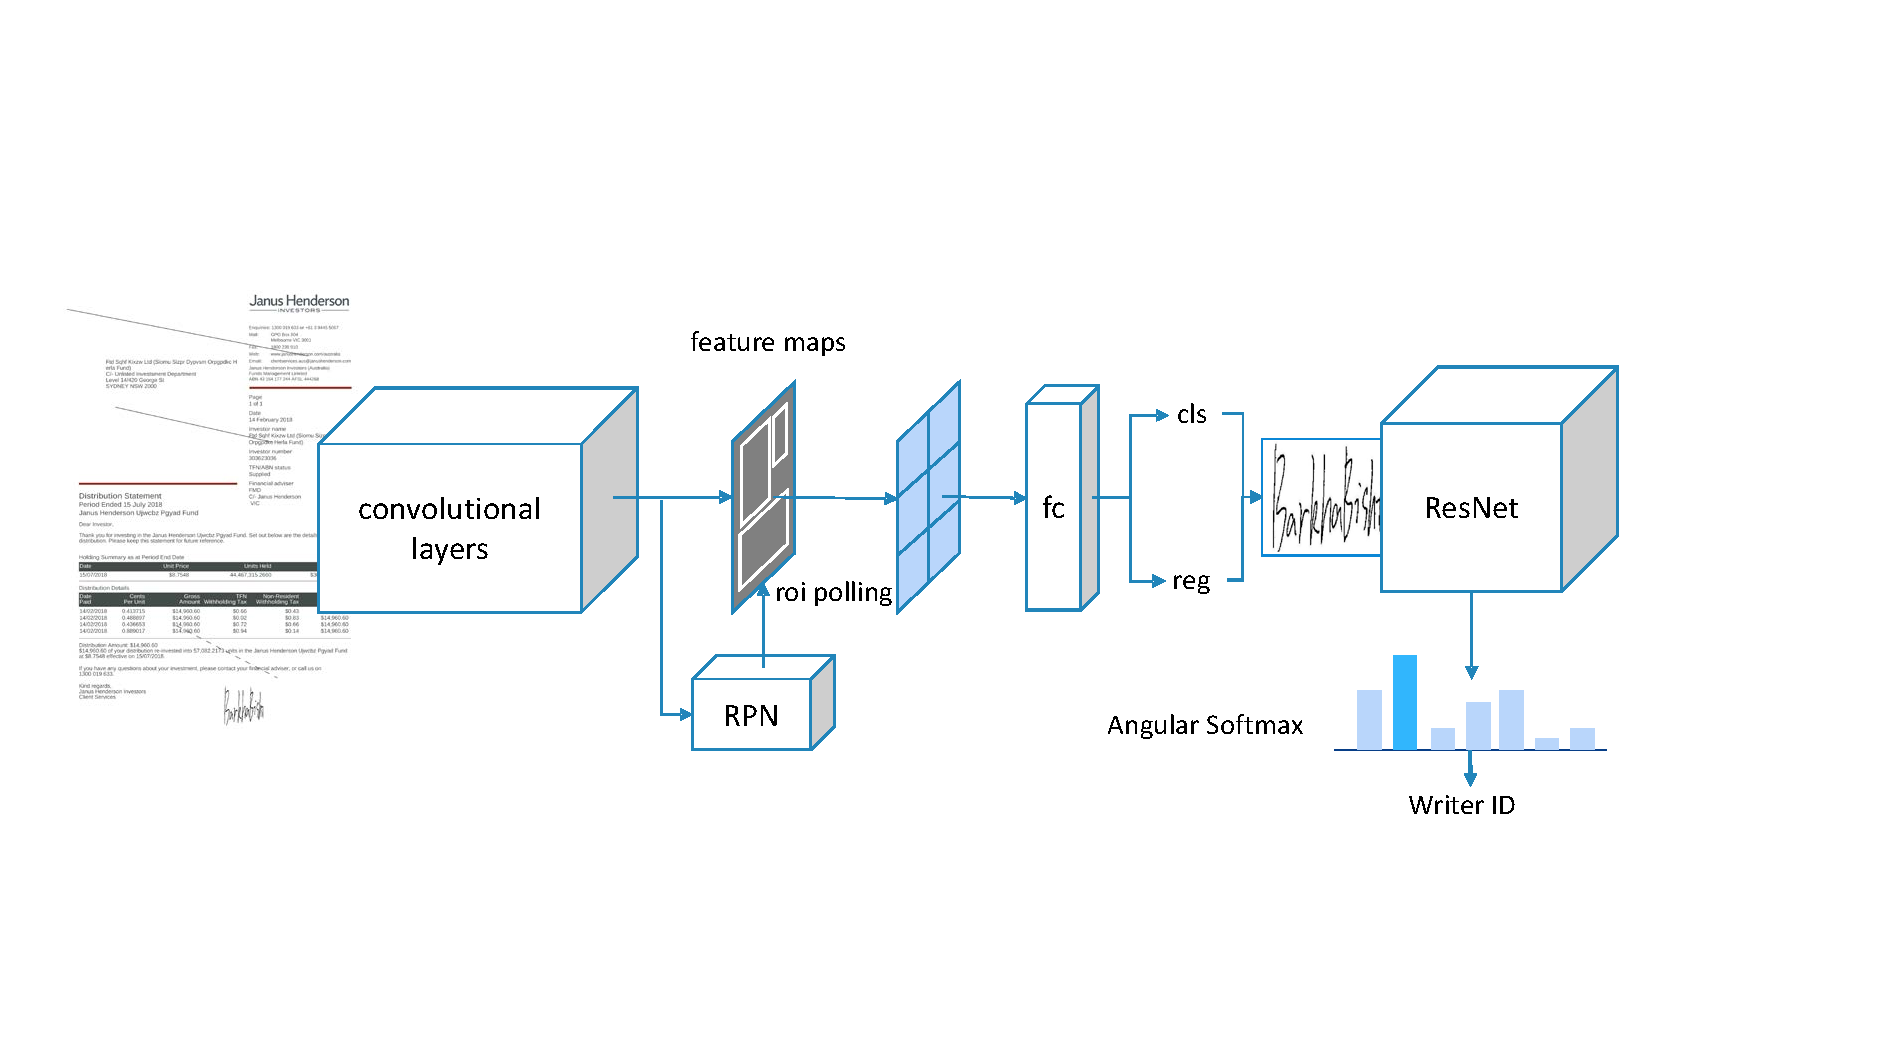
\includegraphics[width=\linewidth]{figure2}
	\caption{Architecture of signature verification model. }
	\label{figure2}
\end{figure*}

\subsection{Signature Detection Model}
Since handwriting features differ vastly from printed texts. It is a relatively simpler task.We employ Faster R-CNN \cite{ren2015faster} with VGG16 \cite{simonyan2014very} to reduce the amount of parameters and save video memory. The architecture is illustrated in Figure \ref{figure2}. Concretely, the model consists three major components. The VGG network is utilized to encode the original image into a latent feature map, and then the feature is fed to the region proposal network (RPN) to generate several region proposals, each of which is a candidate to contain a signature with high likelihood. Finally, both the region proposals and the image feature are taken by the R-CNN subnet as inputs to finetune the precise border of the signature and classify whether the it is a signature block or the background.

\subsection{Writer Verification Model}
As signatures could be forged, it is improper to ''convert'' singatures into names. Instead, with the concern that a signature may belong to an unauthorized writer, we treat this problem as a $k+1$-class ''classification'' task where only $k$ writers are authenticated. Handwriting verification is a difficult problem which remains a challenge. In this paper, we propose to combine Angular Softmax (A-softmax) \cite{liu2017sphereface} and ResNet-50 \cite{he2016deep} as the classification model. A-softmax is an extension of standard softmax which makes the decision boundary more stringent and separated. This way each handwriting can be more likely categorized into a certain class rather close to the boundary between two classes. 

\subsection{Experiments}

\subsubsection*{\rm \textbf{Data Collection}}
As discussed earlier, we use an easy-to-hard training strategy to warm up the training process with a large synthetic dataset. To be specific, we manually collected 86,481 signatures written by 486 individuals. In order to get a robust model to precisely distinguish handwrittings from different individuals, we ask the writers not to sign their own names but to pick five to ten names from a given name list which includes 510 English names, 260 Chinese PinYin names and 264 Indian names, with lengths vary from 5 to 32 characters. All names are signed on a blank form with A4 size. Papers with signatures are sent to a scanner and the scanned signatures are split according to form lines. The average height and width of the signature images are about 140 and 400 pixels respectively. Then we generated 124,445 synthetic faxes which match the layout and style of the real data but with no signatures. The scanned signatures are processed using background elimination and randomly zoomed, twisted and pasted to the white space in synthesized faxes. Each synthetic fax contains 0\textasciitilde5 signatures and the specific statistics are listed in table \ref{stat sig}. We also randomly added several lines as noise into both the synthetic and ''true'' fax images. After preprocessing we obtain training/validation/test sets with 74785/24932/24727 synthetic faxes for signature detection and 72833/5000/8648 respectively for writer verification. The ''true'' data contains 84,000 fax images for training, 18,000 for validation and 18,000 for test respectively.
\begin{table}
	\caption{Statistics of synthetic faxes}
	\label{stat sig}
	\centering
	\begin{tabular}{cc}
		\toprule
		\textbf{\# Signatures} & \textbf{\# Faxes}\\
		\midrule
		0 & 10,000 \\
		1 & 63,939 \\
		2 & 28,520 \\
		3 & 16,784 \\
		4 & 11,688 \\
		\bottomrule
	\end{tabular}
\end{table}

\subsubsection*{\rm \textbf{Evaluation Metrics}}
The two steps are evaluated independently with two different metrics. The performance of signature detection is evaluated by mean average precision (mAP) which is widely used as the standard metric for object detection tasks. Average precision takes both recall and precision into consideration. Formally, AP is computed by the area under precision-recall curve and mAP is the mean value of AP values with respect to all classes. More specifically, a single detection is regarded as correct when intersection-over-union (IOU) is higher than a certain threshold. IOU represents the overlap ratio between the generated candidate bound and the ground truth bound, calculated as the intersection area over the union area. In this paper, the IOU threshold is set to 0.5 which is the most common setting. 

For handwriting verification, we use top-1 and top-5 error rates. Specifically, in the case top-$n$, the model gives $n$ candidates with highest probabilities and the answer is correct if the ground truth label is in the $n$ predictions. 
\subsubsection*{\rm \textbf{Results}}
The mAP score of signature detection is listed in table \ref{signature}. As shown, we find the performance is unsatisfactory for industrial use when we train the model directly on the ''true'' faxes. We argue the reason lies that signatures in real faxes rarely changes on both handwritings and locations, resulting in that the model tends to remember the fixed locations. To improve robustness, we used a warm-up strategy to pre-train the model on a synthetic dataset. The results show a significant improvement of 17.37 mAP score and the high final performance of 91.66 mAP is applicable in production environment.

For writer verification task, we also report the result of a GoogleNet based model \cite{szegedy2015going} with the similar settings. The experimental results listed in table \ref{handwriting} indicates that the ResNet-based model outperforms GoogleNet-based model with 14.32 Top-1 precision and 7.19 Top-5 precision. Finally, the 97.54 Top-5 precision is ready for industrial application with little human examination and intervention.

\begin{table}
	\caption{Performance of signature detection}
	\label{signature}
	\centering
	\begin{tabular}{cc}
		\toprule
		\textbf{Dataset} & \textbf{mAP@0.5} \\
		\midrule
		Synthetic Data & 90.32 \\
		True Data & 74.29 \\
		Synthetic $\rightarrow$ True & 91.66 \\
		\bottomrule
	\end{tabular}
\end{table}

\begin{table}
	\caption{Performance of handwriting verification}
	\label{handwriting}
	\centering
	\begin{tabular}{ccc}
		\toprule
		\textbf{CNN architecture} & \textbf{Top-1 error rate} & \textbf{Top-5 error rate}\\
		\midrule
		GoogleNet & 23.80 & 9.65 \\
		ResNet-50 & 9.48 & 2.46 \\
		\bottomrule
	\end{tabular}
\end{table}


\begin{figure*}[h]
	\centering
	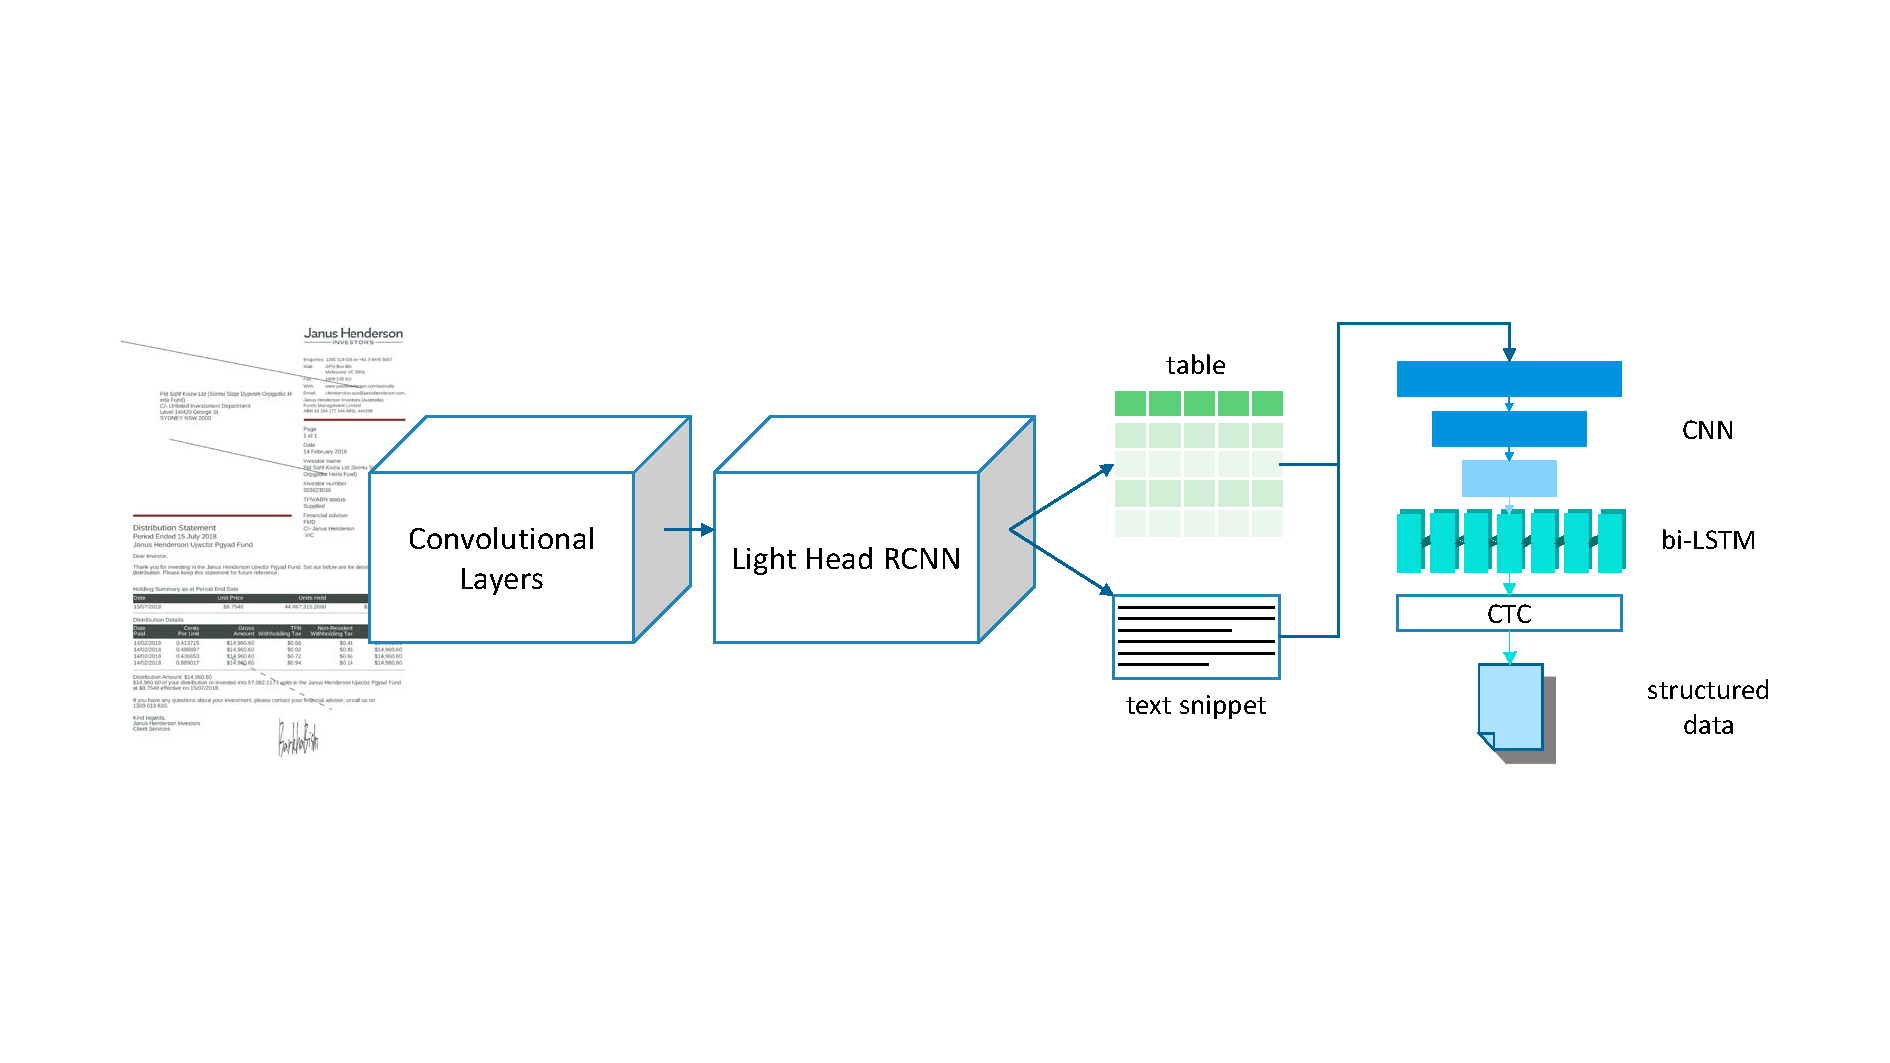
\includegraphics[width=\linewidth]{figure3}
	\caption{Architecture of data extraction model }
	\label{figure3}
\end{figure*}


\section{Data Extraction Models}
Before feeding raw images into data extraction models, we firstly classify faxes into several pre-defined classes according to their business semantics. In practice, the classes are defined with respect to different senders. The process brings two benefits. (i) Since the document style, fonts, layout varies largely across different senders, we can apply multiple data extraction models, each of which only focus on limited types of faxes to improve the accuracy. (ii) with pre-defined layouts, we can summarize each functional areas into some normal forms (i.e., regular expression). This way, the data extraction models only need to recognize raw data from fax images and the extracted texts can also be verified based on the normal forms. In our case, we prepared 51 fax types and employ GoogleNet \cite{szegedy2015going} as the classification model for its flexibility and small size. And we are able to achieve 100\% accuracy finally.

The data extraction process involves two tasks as shown in Figure \ref{figure3}. First, we need to detect areas of each text snippet and in the second step, texts are recognized via OCR. Though existing OCR technology can achieve high accuracy on text recognition, most of them can hardly separate cells in a tabular area and tend to generate text lines sequentially. But data table plays a key role in financial fax processing as it usually contains most intensive useful information. Due to that, our work focuses more on data ingestion from table cells and paragraph texts as shown in Figure \ref{figure5}.


\begin{figure}[h]
	\centering
	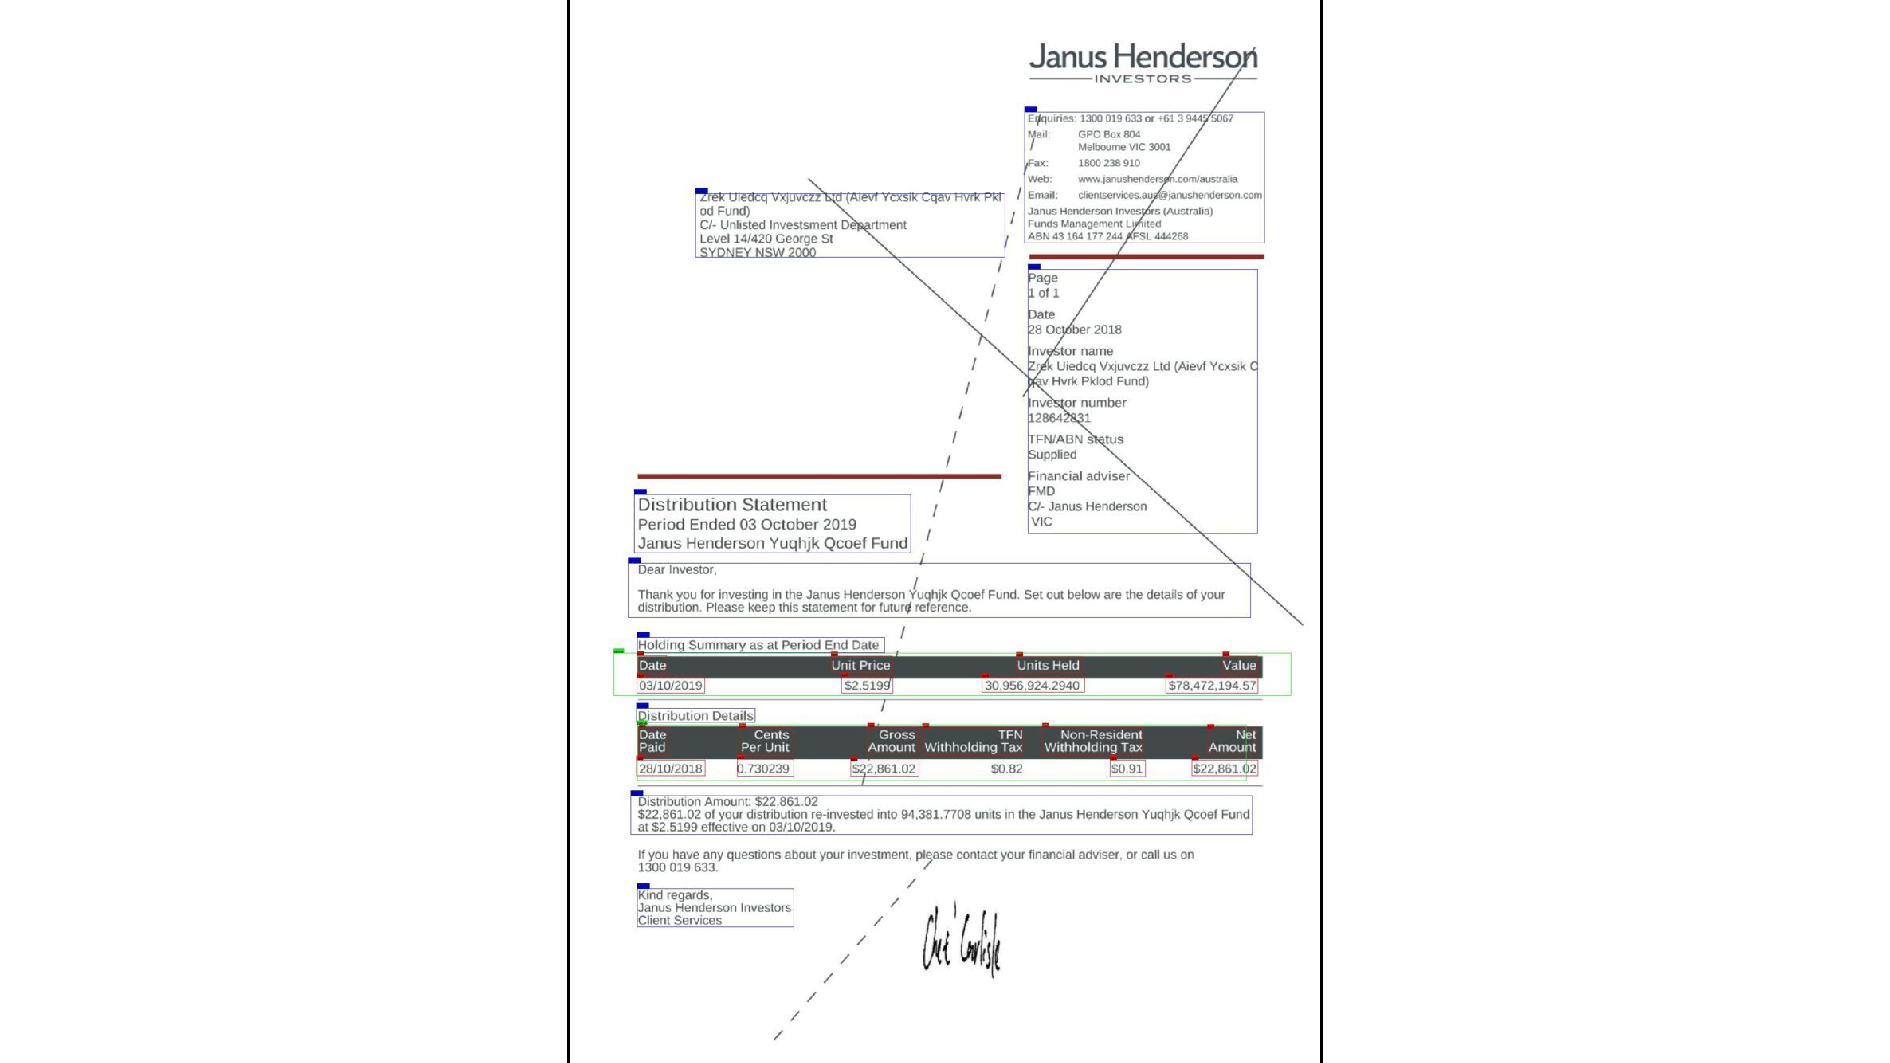
\includegraphics[width=5cm]{figure5}
	\caption{An example of data detection in fax. The text snippets, tables, table cells are highlighted with bleu, green, red bounding rectangles respectively. }
	\label{figure5}
\end{figure}

\subsection{Data Detection Model}
To effectively detect each table cell and text snippet, we apply the state-of-art object detection model Light-Head R-CNN \cite{li2017light} for this task. Light-Head R-CNN is an extension of Faster R-CNN with higher detection accuracy and speed. Moreover, we choose ResNet-101 in \cite{he2016deep} as the CNN structure for higher detection performance.

As in our experiments, we found that directly training the models with three classes (table cells, text snippets and background) can hardly achieves a satisfactory result. The reason is that texts in table and other paragraphs are often in some fonts, sizes, and peripheral regions are usually blank, which limits the model to distinguish table and paragraphs. To address this problem, we add a new class "table" into the detection problem during training which can improve detection accuracy of cell texts by explicitly provide the relative relationship between tables and text paragraphs.

Another problem for the data detection model is that NMS (non maximal suppression) can result in overlapped candidate regions when $NMS\_THRESHOLD$ is less than 1. It is common for general object detection but can result in duplicate text recognized in our system. Therefore, we just set $NMS\_THRESHOLD$ to 1 and combine all overlapped regions into one area. The algorithm for removing overlapped regions is detailed in Algorithm \ref{algorithm2}.

\begin{algorithm}[htb]
	\caption{Removing Overlapped Candidate Regions}
	\label{algorithm2}
	\raggedright
	\KwIn{Candidate Regions $regs$ of the same class after NMS with $NMS\_THRESHOLD=1$; The length of $regs$ is $len$}
	
	\KwOut{Final region array $outs$ with length $len$}
	sort $regs$ according to the top/left coordinates from top left corner to bottom right.\\
	Initialize boolean array $known$ with length $len$ by setting all elements to $False$.\\
	Initialize boolean array $overlap$ with length $len$ by setting all elements to $False$.\\
	
	\For{$i=0; i<len; i++$}{
		\If{$overlap[i]==True$}{continue}
		Set $known[i]=True$\\
		Get the coordinates of top left corner and bottom right corner of $regs[i]$: $xmin_{i}, ymin_{i}, xmax_{i}, ymax_{i}$\\
		\For{$j=0; j<len; j++$}{
			\If{$overlap[i]==True$ or $known[i]==True$}{continue}
			Get the coordinates of top left corner and bottom right corner of $regs[j]$: $xmin_{j}$, $ymin_{j}$, $xmax_{j}$, $ymax_{j}$\\
			Compute the interesection area of $regs[i]$ and $regs[j]$ as $inter$.\\
			\If{$inter>0$}{
				$overlap[j]=True$\\
				Set $xmin_{i}=min(xmin_{i},xmin_{j})$\\
				Set $ymin_{i}=min(ymin_{i},ymin_{j})$\\
				Set $xmax_{i}=max(xmax_{i},xmax_{j})$\\
				Set $ymax_{i}=max(ymax_{i},ymax_{j})$\\
			}	
		}
		Set $xmin_{i}, ymin_{i}, xmax_{i}, ymax_{i}$ to $outs[i]$
	}
\end{algorithm}

\subsection{Text Recognition Model}
The OCR model is convolutional recurrent neural network (CRNN) \cite{shi2017end} in this task. The model consists of a deep CNN, a bi-directional recurrent network (bi-RNN) with long short term units (LSTM) and a connectionist temporal classification (CTC) \cite{graves2006connectionist} output layer. Similar to the detection model, the CNN body is utilized to extract the feature map of the original image and the structure is VGG-16 for its good performance on transfer tasks. The bi-RNN model on top of the CNN is responsible to generate the characters sequentially. CTC output layer is responsible to compute the probability of each output label generated by bi-LSTM by marginalizing
over the set of all possible alignments paths, which is appropriate to find the local optimum sequence among blanks and duplicate characters.
\subsection{Experiments}
\subsubsection*{\rm \textbf{Data Collection}}
For the data detection task, as shown in Figure \ref{figure4}, the layout of real fax is quite complex and we find it is hard to converge when we directly train the detection model on the real dataset. To address this issue, we construct a synthesized dataset, the fax image in which is much simpler in terms of layout and drawing format, but more various in density of table/text cells, fonts and sizes. Since the features in structures at coarse-grained level (layouts and formats) is easy to capture, the model can converge quickly, and the introduced fine-grained variabilities (location and fonts) can bring robustness to the model. A synthesized fax may have multiple text snippets, tables and multiple signatures. The size, location, font and rotation of each text area are all random. In this way, are are capable to obtain a large-scale labeled dataset with 80,000 samples. We split the dataset with ratio 70\%/15\%/15\% for training/validation/test respectively. 

For text recognition model, we simply mix the images of table cells and text snippets from both the synthesized and true datasets. It should be noted proper preprocessing process can greatly improve the recognition accuracy. Specifically, we preprocessed the cell and text snippet images with such methods as enhance normalization, text smoothing with threshold 50\%, grayscaling, background cleaning with filter size 25, background trimming, sharpening and border padding. The preprocessing methods are verified to be effective in our experiments.

\subsubsection*{\rm \textbf{Evaluation Metrics}}
The data detection model is evaluated with mAP metric which is the same with the signature detection model. For text recognition, we propose a hybrid evaluation metric namely Modified Word Accuracy which is more appropriate to measure how much manual labor has been reduced by our system. To be specific, different from existing work \cite{borisyuk2018rosetta, shi2017end} which uses fragment accuracy and edit distance for evaluation independently, we combine the two metrics. First we set score 1 to all correctly recognized words. Then for the incorrect words, the score is defined as the ratio of edit distance between the correct and incorrect words to the length of the true word. 

\subsubsection*{\rm \textbf{Results}}
The main results of data detection tasks are shown in Table \ref{tabel_detection}. It can be observed that our warm up strategy is quite effective in the task. The model is capable to achieve high performance on the synthesized dataset with 90.71 mAP for the simple coarse-grained layouts and formats. However, the mAP drops sharply when trained on the true data directly which is far from industrial application. With the warm-up strategy, the final mAP on the true data is 98 mAP which is even higher than the results on the synthetic data. The reason is that the real dataset has less variability than the synthesized one but the complex drawing format makes the CNN architecture difficult to map the original fax image into latent space and it is where our warm up strategy works.

For the text recognition tasks, we can observe the clear gap between the two strategies with or without image preprocessing. Finally, the text recognition model achieves the industrial applicable results of 96.41 accuracy. In this way, only one or two human checkers are
needed to check whether the recognized tables and texts are correct or not. Manual work on typing the entire texts of a fax is never needed.

\begin{table}
	\caption{Performance of data detection}
	\label{tabel_detection}
	\centering
	\begin{tabular}{ccccc}
		\toprule
		\multirow{2}{1cm}{\textbf{Dataset}} & \multirow{2}{0.8cm}{\textbf{mAP}} & \multicolumn{3}{c}{\textbf{AP}}\\
		\cline{3-5}
		& & \textbf{Text Snippet} & \textbf{Table} & \textbf{Cell}\\
		\midrule
		Synthetic Data & 90.71 & 90.43 & 90.66 & 91.03 \\
		True Data & 53.86 & 48.33 & 49.02 & 64.24 \\
		Synthetic $\rightarrow$ True & 98.00 & 95.21 & 99.99 & 98.81 \\
		\bottomrule
	\end{tabular}
\end{table}

\begin{table}
	\caption{Performance of text recognition}
	\label{text_recognition}
	\centering
	\begin{tabular}{cc}
	\toprule
	\textbf{preprocessing} & \textbf{Modified Word Accuracy} \\
	\midrule
	No & 88.75 \\
	Yes & 96.41 \\
	\bottomrule
	\end{tabular}
\end{table}


\section{Deployment}
\subsection{Deployment Strategy}

\subsection{Incremental Learning with Author Feedbacks}
As a online system, author feedbacks received are extremely valuable for model refining continuously. Every author feedback can be regarded as a new training sample. Since all the machine learning models in our system are built with neural networks, it can be naturally fine-tuned to adapt to only the feedback samples but need not re-trained on whole training data. However, directly training networks on new data may lead to catastrophic forgetting, that is the network will forget previously learned knowledge. To address this issue, we, with inspiration from existing works \cite{shmelkov2017incremental, yuan2018text}, propose to fine-tune the models with distillation loss.

Specifically, given a trained model $M$ with fixed parameters, the first step is to make a copy $M^{*}$ from $M$. At each timestep during training, we first sample a batch of data $T_{o}$ from $D$. Then we divide both $M$ and $M^{*}$ into several groups and compute the distillation loss on $T_{f}$ as:

\begin{equation}
\label{eqn_dist}
	\mathcal{L}_{dist} = \sum_{l=1}^{L}||\phi_{M}^{l}(T_{o})-\phi_{M^{*}}^{l}(T_{o}) ||_{1},
\end{equation}
where $||\cdot||$ is L1 norm, $\phi_{M}^{l}$ and $\phi_{M^{*}}^{l}$ denotes the output of the $l$-th group of $M$ and $M^{*}$ respectively. For object detection models (faster rcnn and light-head rcnn), the groups are divided according to the function of different components, including feature extractor, region proposal network and R-CNN subnet. The feature extractor CNN is further separated into several blocks with respect to the pooling processing (VGG) or residual blocks (ResNet) and classification models share this group definition. To adapt the model to the new feedback data, we train $M^{*}$ on $T_{f}$ by minimizing the standard classification/detection loss $\mathcal{L}_{task}$. The final loss is computed as:

\begin{equation}
\mathcal{L}=\mathcal{L}_{task} + \alpha\cdot\mathcal{L}_{dist}
\end{equation}
where $\alpha$ is a hyper-parameter to control the ratio between distillation loss and standard loss. The algorithm is detailed in Algorithm \ref{algorithm1}.


\begin{algorithm}[htb]
	\caption{Incremental Learning with Author Feedbacks}
	\label{algorithm1}
	\raggedright
	\KwIn{Trained Model $M$; Author feedback set $D_{f}$; Original training dataset $D$; Batch size $B$; New data rate $p$; Weight of distillation loss $\alpha$, Training algorithm $A$}
	
	\KwOut{Trained New Model $M^*(\theta)$}
	\While{not converge}{
		Random sample a training batch $T$, including $B\times p$ samples from $D_f$ as $T_{f}$ and $B\times (1 - p)$ samples from $D$ as $T_{o}$ respectively \\
		Compute distillation loss $\mathcal{L}_{dist}$ on $T_{o}$ as Eqn. \ref{eqn_dist}\\
		Compute task loss $\mathcal{L}_{task}$ on $T_{f}$ \\
		Update model paramter $\theta$ with $A$ by minimizing training loss $\mathcal{L}=\mathcal{L}_{task} + \alpha\cdot\mathcal{L}_{dist}$
	}
\end{algorithm}

\section{Conclusion and Future Work}

In this paper, we present a system that automatically parses fax images into the structured formatted data. The system consists of three major functional components: signature verification, template classification and data extraction. On all the tasks, the system has achieved high accuracy and significantly reduce human labor.

Moreover, we also propose a detailed interactive training strategy. With this approach, the system is able to absorb the effective knowledge from author feedback and in turn fine-tune the machine learning models continuously.

In the future, we plan to extend the system in two aspects. First, we will investigate the methods to precisely convert tabular data into the formats we want. It is a challenging task for the statement and layout vary largely in different companies. Second, we are interested in improving the quality and accuracy of the existing models.


\bibliographystyle{ACM-Reference-Format}
\bibliography{kdd}

\end{document}
